\documentclass[tikz,border=2pt]{standalone}
\usepackage{amsmath,amssymb}
\usepackage{tikz}
\usetikzlibrary{arrows.meta}

\begin{document}
% An undirected network: edges have no orientation and may be traversed either way.
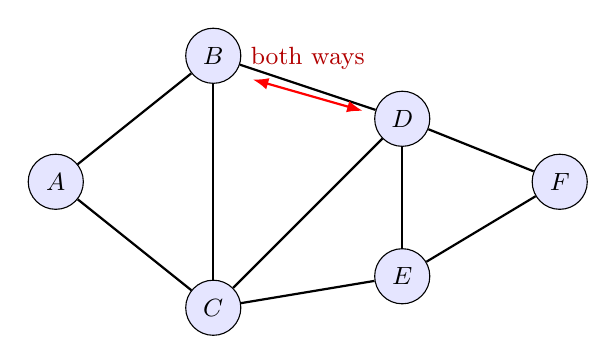
\begin{tikzpicture}[every node/.style={font=\small}, >={Latex[length=2mm]}, v/.style={draw, circle, fill=blue!10, minimum size=7mm, inner sep=0pt}]
	\node[v] (A) at (0,0) {$A$};
	\node[v] (B) at (2,1.6) {$B$};
	\node[v] (C) at (2,-1.6) {$C$};
	\node[v] (D) at (4.4,0.8) {$D$};
	\node[v] (E) at (4.4,-1.2) {$E$};
	\node[v] (F) at (6.4,0) {$F$};
	\foreach \a/\b in {A/B, A/C, B/C, B/D, C/D, C/E, D/E, D/F, E/F} {\draw[thick] (\a) -- (\b);}
	\draw[<->, red, thick] (2.5,1.3) -- (3.9,0.9);
	\node[red!70!black, font=\small, anchor=south] at (3.2,1.3) {both ways};
	\end{tikzpicture}
\end{document}
